\section{Datasets}
\label{sec:datasets}
  When testing the bootstrapping loss function and curriculum learning, as well as measuring the performance of the road detection system, two datasets have been utilized. Both datasets involve the task of semantic segmentation of images, more precisely, the task of extracting roads from aerial images. The first dataset, the Massachusetts Roads Dataset, provided by \cite{MnihThesis}, has been used in several works. The second dataset, the Norwegian Roads Dataset, was specifically made for this thesis, and was generated from publicly available data. Differences, similarities, and challenges of employing these datasets will be further discussed below.\\

\subsection{Massachusetts Roads Dataset}
The Massachusetts Roads Dataset contains aerial images depicting urban, suburban, and rural areas in the state of Massachusetts, USA. In all, the dataset consists of 1171 aerial images, where each image is $1500\times 1500$ pixels in size. 1108 of these images have been randomly assigned to the training set. The remaining 49 and 14 images can be found in the test and validation set. The dataset covers an area of approximately 2600 square kilometers in total, which gives a \ac{GSD} of 1.0 meter per pixel.\\

Each aerial image has an accompanying identically sized binary label image, which indicates whether a pixel in the aerial image belongs to either the road or non-road class. Road centerline vectors retrieved from the OpenStreetMap project were used to generate the label images. The vectors were rasterized as white lines with a line thickness of 7 pixels \citep{MnihThesis}, which, based on the \ac{GSD}, is equivalent to 7 meters on the ground. An aerial image and label image pair from this dataset can be seen in Figure \ref{fig:mass_roads_example}.\\

\begin{figure}
\begin{subfigure}{0.48\textwidth}
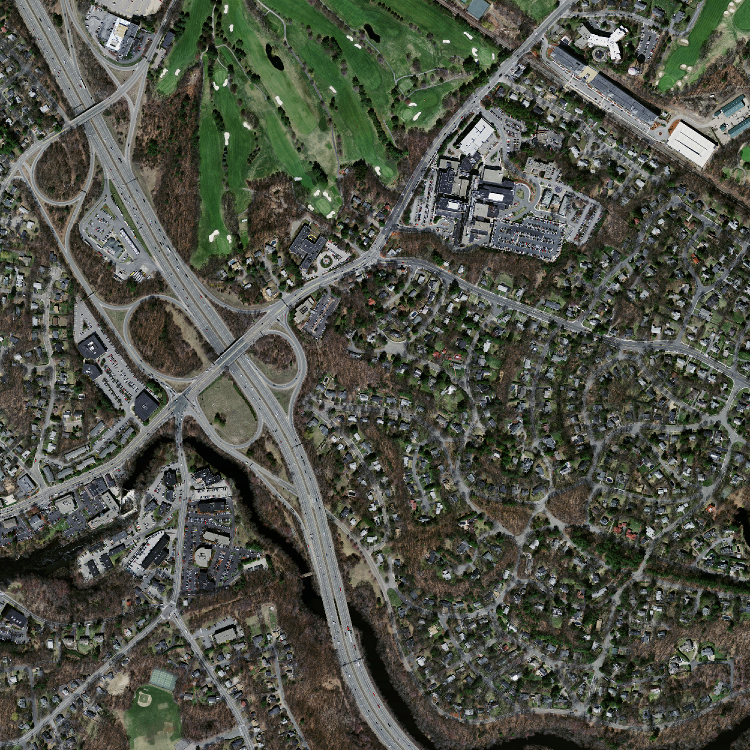
\includegraphics[width=\linewidth]{figs/datasets/Mass_roads_data_example2.png}
\caption{Aerial image.} \label{fig:mass_roads_example_data}
\end{subfigure}
\hspace*{\fill} % separation between the subfigures
\begin{subfigure}{0.48\textwidth}
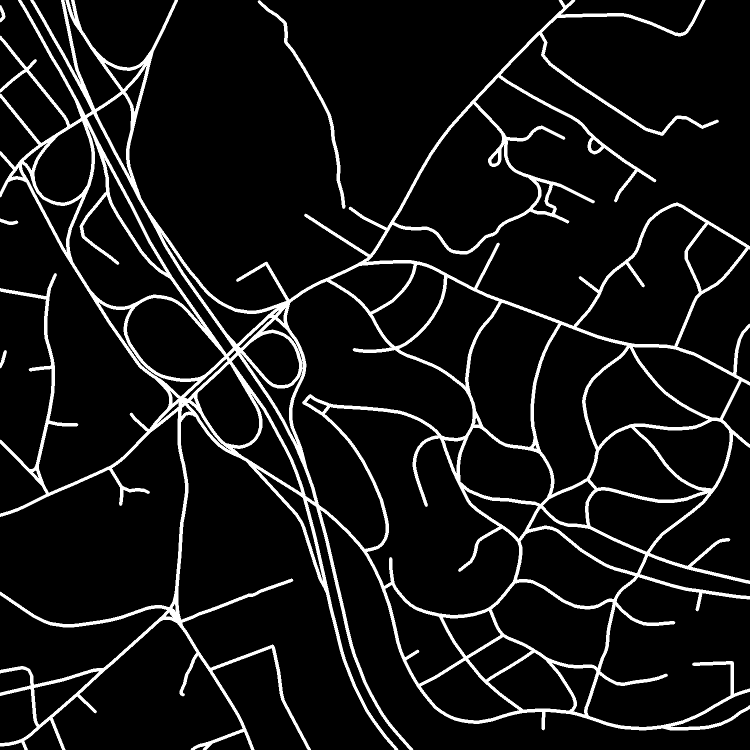
\includegraphics[width=\linewidth]{figs/datasets/Mass_roads_label_example2.png}
\caption{Label image.} \label{fig:mass_roads_example_label}
\end{subfigure}
\hspace*{\fill} % separation between the subfigures
\caption[The Massachusetts Roads Dataset]{Image and label example taken from test set in the Massachusetts Roads Dataset.} \label{fig:mass_roads_example}
\end{figure}


There are many reasons for using this dataset to conduct experiments related to the research questions.  The task involves semantic segmentation of roads based exclusively on aerial color images. This is arguably a hard task, and might justify the use of a large model for training, such as a \ac{CNN}. The dataset has also been used in other works, which enables comparison of the results obtained in this thesis to the results obtained in other works. Additionally, the labels have been generated from existing map data, and therefore contain many instances of naturally occurring inconsistent labeling. This is compelling in relation to the research questions of this thesis.\\

Aerial image datasets typically suffer from two distinct types of label noise, which \cite{Mnih_aerial_images_noisy} have named omission and registration noise. The dataset is generated from existing map data, which can have some deficiencies when coupled with supervised learning. There are many instances of omission noise in this dataset, where smaller roads and parking areas have not been marked as road class pixels in the label images. These omissions are most likely perfectly acceptable for map purposes, but might negatively impact the performance of a classifier.  For instance, unlabeled paved areas that share a high spectral similarity to roads could be considered inconsistently labeled. These label errors might compel the classifier to minimize the loss by learning complicated distinctions between surfaces that are essentially the same thing.\\

There are also instances of registration noise in this dataset. This happens when there are misalignments between the roads found in the aerial images and the road centerline vectors from the map data. Additionally, the road centerline vectors have, in many cases, been rasterized with the incorrect line thickness, which might cover too much or not enough depending on the road's lane width. The result is a lot of aerial image pixels that have been assigned the wrong class, which might impact the learning procedure negatively. Slightly misaligned road centerline vectors probably do not affect map products much, whereas they create a lot of inconsistent examples in a machine learning dataset.


%\subsection{Massachusetts Roads Dataset}

\subsection{Norwegian Roads Dataset}
In addition to the Massachusetts Roads Dataset, the proposed methods have been tested with the Norwegian Roads Dataset. This dataset was constructed from aerial images retrieved from Kartverket, which depicts both rural, suburban, and urban areas from different locations in Norway. The entire dataset consists of 1225 aerial images, each being $1536\times 1536$ pixels in size. 1100 of them have been randomly assigned to the training set, 75 to the test set, and the remaining images were put in the validation set. Even though there are more aerial images in this dataset compared to the Massachusetts Roads Dataset, it only covers an area of around 1910 square kilometers. This is due to a much lower \ac{GSD} of about 0.66 meters per pixel. \\


The label images in this dataset have been generated from road centerline vectors found in the publicly available topographic vector database, N50, provided by \cite{Kartverket}. Unlike the Massachusetts Roads Dataset, the centerline vectors have been rasterized with a variable line thickness. This is possible because all road segments in N50 have a set of properties, which can be utilized to determine a custom line thickness. The actual thickness of each road type has been based on numbers found in a road specification manual published by the Norwegian Public Roads Administration \citep{Norwegian_road_manual}. The road segment properties and line thickness for each road type are listed in Table \ref{tab:road_rules}. Roads that are underground and cannot be seen from aerial imagery have also been removed from the rasterized label images.\\

The aerial images have been taken from over 30 different locations in Norway, and offers a large variety of topographical features. There are images depicting coastlines, rivers, mountain terrains, snow, cultivated land, and forests. Compared to Massachusetts Roads Dataset, the aerial images of this dataset have been sampled from a much larger area. Furthermore, the aerial images might present a challenge in terms of image quality. Some of the images vary in terms of color balance and image contrast. There are also aerial images that have been stitched together from images captured by aerial surveys conducted at different occasions.\\

The quality of the generated label maps might also present a challenge to a machine learning algorithm. There are both omission and registration errors present in many of the label images. Compared to the Massachusetts Roads Dataset there is a much higher degree of registration noise. The road centerlines in N50 generally appear more coarse, and result in less overlap between roads in the aerial image and the raster lines in the label image. This is especially evident in road centerline vectors for divided highways. Instead of having centerline vectors for both roadways, there is only one placed between the roadways on the median. Visual examples of missing and misplaced labels can be seen in Figure \ref{fig:norwegian_roads_examples_n50}.\\

\begin{figure}[h]
\begin{subfigure}{0.31\textwidth}
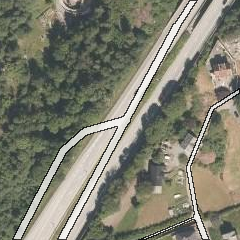
\includegraphics[width=\linewidth]{figs/datasets/nor_examples/1191_highway_n50.png}
\caption{Divided highways.} \label{fig:norwegian_roads_highway_n50}
\end{subfigure}
\hspace*{\fill} % separation between the subfigures
\begin{subfigure}{0.31\textwidth}
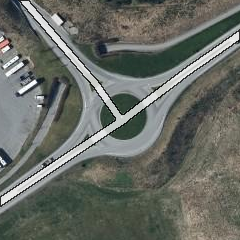
\includegraphics[width=\linewidth]{figs/datasets/nor_examples/1177_roundabout_n50.png}
\caption{Roundabout.} \label{fig:norwegian_roads_roundabout_n50}
\end{subfigure}
\hspace*{\fill} % separation between the subfigures
\begin{subfigure}{0.31\textwidth}
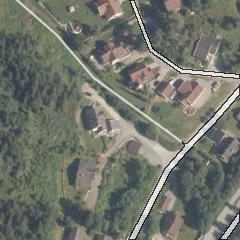
\includegraphics[width=\linewidth]{figs/datasets/nor_examples/1157_missing_n50.png}
\caption{Private road.} \label{fig:norwegian_roads_missing_n50}
\end{subfigure}
\hspace*{\fill} % separation between the subfigures
\caption[Inconsistent labeling in the Norwegian Roads Dataset N50]{Examples of inconsistent labeling found in the Norwegian Roads Dataset N50.} \label{fig:norwegian_roads_examples_n50}
\end{figure}

In addition to the set of label images generated from N50, the dataset also includes an alternate set of label images generated from the road centerline vector database, Vbase \citep{Kartverket_vbase}. This database has more accurate road centerline vectors. There are still omission and registration errors present in this label image set, but to a less extent. Surfaces that share spectral similarities to asphalt, such as private roads and parking areas, have not been marked, similar to the Massachusetts Roads Dataset. The difference in accuracy between N50 and Vbase can be seen by comparing Figure \ref{fig:norwegian_roads_examples_n50} and Figure \ref{fig:norwegian_roads_examples_vbase}. A minor downside of using this alternate vector database is that Vbase provides fewer road segment properties, which have resulted in a smaller set of line thicknesses applied to the label images.\\

\begin{figure}[h]
\begin{subfigure}{0.31\textwidth}
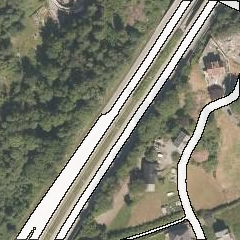
\includegraphics[width=\linewidth]{figs/datasets/nor_examples/1191_highway_vbase.png}
\caption{Divided highways.} \label{fig:norwegian_roads_highway_vbase}
\end{subfigure}
\hspace*{\fill} % separation between the subfigures
\begin{subfigure}{0.31\textwidth}
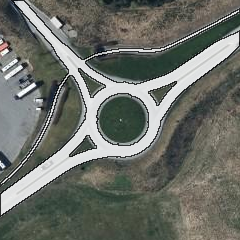
\includegraphics[width=\linewidth]{figs/datasets/nor_examples/1177_roundabout_vbase.png}
\caption{Roundabout.} \label{fig:norwegian_roads_roundabout_vbase}
\end{subfigure}
\hspace*{\fill} % separation between the subfigures
\begin{subfigure}{0.31\textwidth}
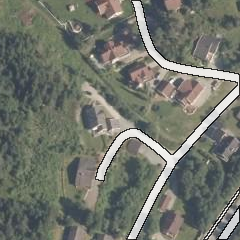
\includegraphics[width=\linewidth]{figs/datasets/nor_examples/1157_missing_vbase.png}
\caption{Private road.} \label{fig:norwegian_roads_missing_vbase}
\end{subfigure}
\hspace*{\fill} % separation between the subfigures
\caption[Road centerline vector quality of Vbase]{Examples of road centerline vector quality in Vbase.} \label{fig:norwegian_roads_examples_vbase}
\end{figure}

\begin{table}[htp]
\caption[Raster line thicknesses for the Norwegian Roads Dataset]{Raster line thickness and road segment filtering rule for each type of road. A margin of 10\% is removed from the line thicknesses, which are based on numbers found in the road specification manual.}
\begin{center}
\begin{adjustbox}{max width=\textwidth}
\begin{tabular}{+l ^l ^r}\hline
		 \rowstyle{\bfseries}
 		 Road type & Road segment property & Line thickness\\\hline
 		 Dirt road & OBJTYPE=Traktorveg & 2.50 m\\
 		 Trail & OBJTYPE=Sti & 1.50 m\\
 		 pedestrian road & OBJTYPE=GangSykkelveg & 2.25 m\\
 		 Highway & MOTORVEGTYPE=motorveg & 10.80 m\\
 		 International E-road network & VEGKATEGORI=E & 6.30 m\\
 		 Norwegian national road & VEGKATEGORI=R & 5.85 m\\
 		 municipal road & VEGKATEGORI=K & 4.95 m\\
 		 Private road & VEGKATEGORI=P & 3.50 m\\\hline
\end{tabular}
\end{adjustbox}
\end{center}
\label{tab:road_rules}
\end{table}

The dataset was constructed by using QGIS, an open source geographic information system application. The application enables viewing and editing of map data, but also provides a Python interface. A script to create label images was developed, taking the map coordinates associated with each corner of an aerial image, and generating a raster image of road centerline vectors found inside that area. The resulting raster images can be used as target maps in supervised learning. \\

\begin{figure}
\begin{subfigure}{0.32\textwidth}
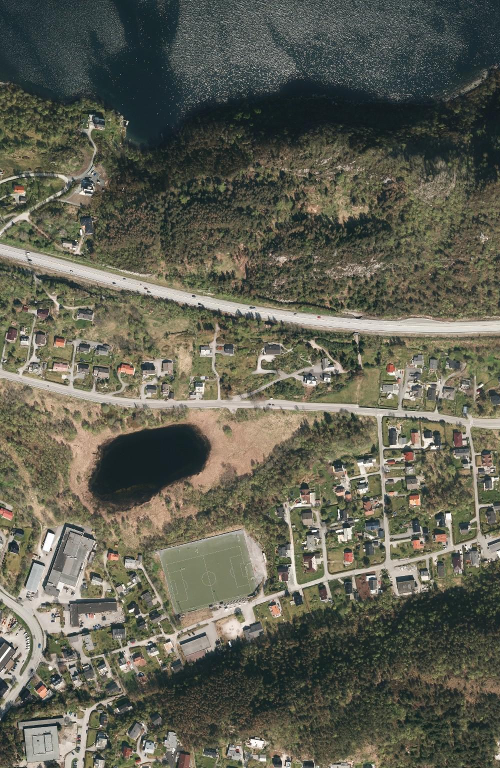
\includegraphics[width=\linewidth]{figs/datasets/Norwegian_roads_data_example2.png}
\caption{Aerial image} \label{fig:norwegian_roads_example_data}
\end{subfigure}
\hspace*{\fill} % separation between the subfigures
\begin{subfigure}{0.32\textwidth}
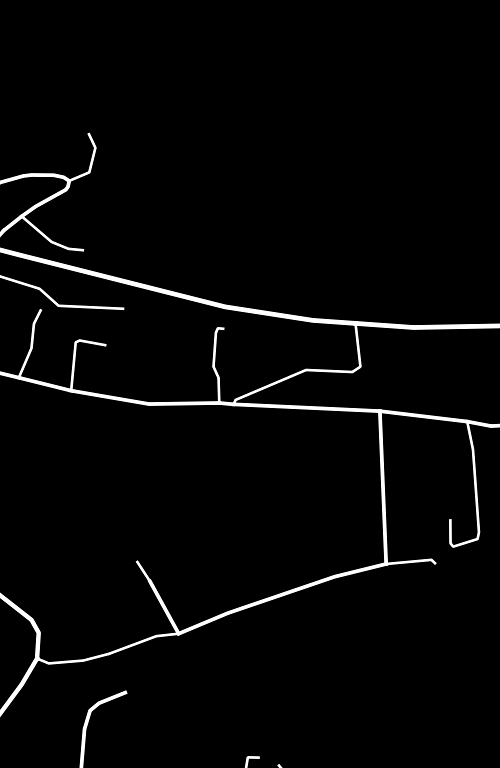
\includegraphics[width=\linewidth]{figs/datasets/Norwegian_roads_label_example2.png}
\caption{Label image} \label{fig:norwegian_roads_example_label}
\end{subfigure}
\hspace*{\fill} % separation between the subfigures
\begin{subfigure}{0.32\textwidth}
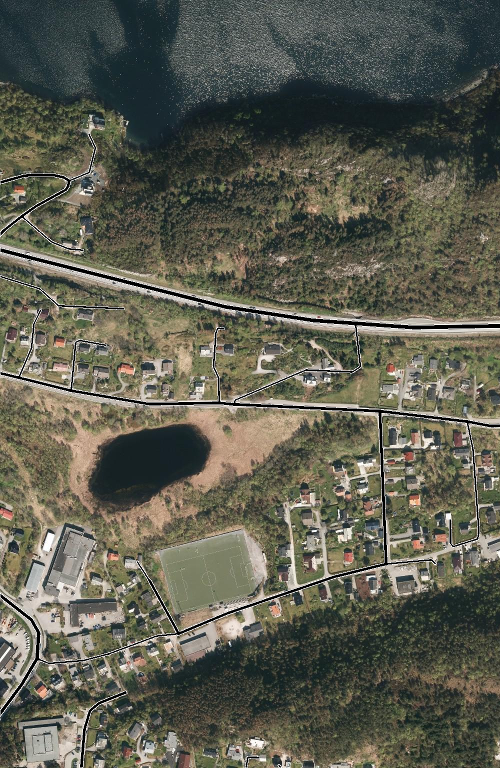
\includegraphics[width=\linewidth]{figs/datasets/Norwegian_roads_overlay_example2.png}
\caption{Overlay image} \label{fig:norwegian_roads_example_overlay}
\end{subfigure}
\hspace*{\fill} % separation between the subfigures
\caption[Example from Norwegian Roads Dataset N50]{Example from test set in Norwegian Roads Dataset N50.} \label{fig:norwegian_roads_example}
\end{figure}

An aerial image and its corresponding label image from the Norwegian Roads Dataset N50 can be seen in Figure \ref{fig:norwegian_roads_example}. Figure \ref{fig:norwegian_roads_example_overlay} shows the same label image superimposed on the aerial image. Observe that some roads are missing from the label image, as well as the ground truth not covering the roads properly. \\
